% Preamble
\documentclass[11pt]{beamer}
% Add xcolor with dvipsnames to define structure colors
\usepackage[dvipsnames]{xcolor}
\mode<presentation>{
  \usetheme{Madrid}
  \usecolortheme[named=Periwinkle]{structure}
  \useoutertheme{shadow}
  \setbeamertemplate{navigation symbols}{}
  \setbeamertemplate{headline}{}
}
\usepackage[italian]{babel}
\usepackage[utf8]{inputenc}
\usepackage[T1]{fontenc}
\usepackage{graphicx}
\hypersetup{
  pdftitle={Performance Analysis for Projection-Correction Methods in Motion Deblurring Problems},
  pdfauthor={Sara Casadio, Enrico Ferraiolo, Giovanni Savoca}
}

% Title and Author
\title[Project Correction]{Performance Analysis for Projection-Correction Methods in Motion Deblurring Problems}
\author[Gruppo 20]{Sara Casadio, Enrico Ferraiolo, Giovanni Savoca}
\institute[Istituzione]{%
  Alma Mater Studiorum - Università di Bologna \\
  Corso di Laurea in Informatica
}
\date{\today}

\begin{document}

% Title Frame
\begin{frame}
  \titlepage
\end{frame}

% Section 1
\section{Descrizione del problema}
\subsection{Problem Description}
\begin{frame}{Problem Description}
  \begin{itemize}
    \item The project analyzes the performance of two \textbf{Projection-Correction} algorithms for reconstructing medical images affected by \textbf{motion blur}.
    \item The studied algorithms are:
    \begin{itemize}
      \item \textbf{Diffusion Posterior Sampling (DPS)}
      \item \textbf{Regularization by Denoising with Diffusion (RED-Diff)}
    \end{itemize}
    \item Both methods are based on \textbf{pre-trained diffusion models}.
    \item Objective: evaluate the effectiveness of these methods in recovering degraded images.
  \end{itemize}
\end{frame}

% Section 2
\section{Approccio di risoluzione con dps e rediff + modello diffusivo}
\input{capitoli/ApproccioRisoluzione.tex}

% Section 3
\section{Dataset}
\subsection{Mayo Clinic CT Dataset}

\begin{frame}{Mayo Clinic CT Dataset}
  \begin{itemize}
    \item Released by the \textbf{Mayo Clinic} for research purposes.
    \item Contains chest \textbf{Computed Tomography (CT)} scans.
    \item Images are in \textbf{grayscale (black and white)} format.
    \item Focus on \textbf{lung nodules} and early detection of \textbf{lung cancer}.
    \item Widely used in machine learning and AI medical imaging research.
  \end{itemize}
  \vspace{0.5cm}
  \begin{center}
    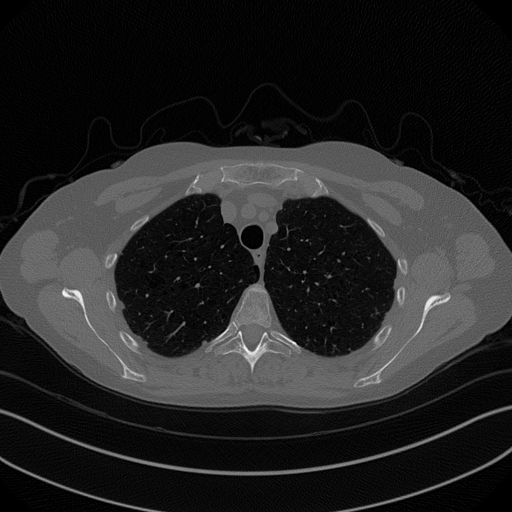
\includegraphics[width=0.25\linewidth]{media/2.png}
    \hspace{0.3cm}
    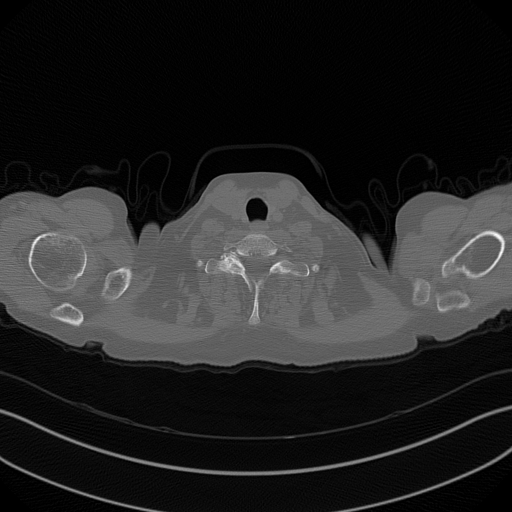
\includegraphics[width=0.25\linewidth]{media/3.png}
    \hspace{0.3cm}
    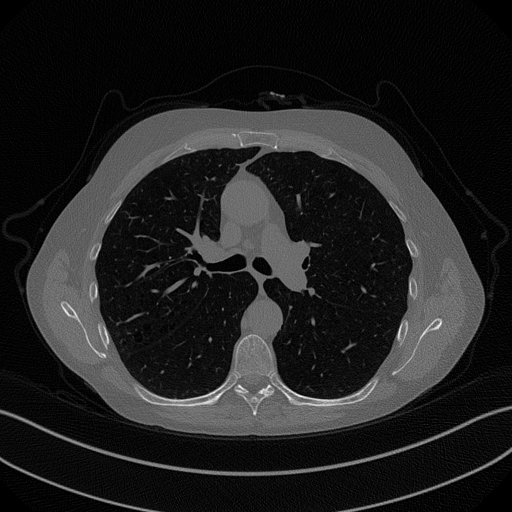
\includegraphics[width=0.25\linewidth]{media/100.png}
  \end{center}
\end{frame}

\begin{frame}{Preprocessing and Augmentation}
  \begin{itemize}
    \item All CT images were preprocessed and resized to a fixed dimension of \textbf{128 × 128 pixels}.
    \item This standardization ensures consistency for input into deep learning models.
    \item The dataset was \textbf{augmented} to avoid overfitting and improve model generalization (detailed later).
  \end{itemize}
\end{frame}

% Section 4
\section{organizzazione della repository}
\subsection{Sottosezione 2.1}
\begin{frame}{Sottosezione 2.1}
  % Contenuto qui
\end{frame}

% Section 5
\section{architettura della rete diffusiva}
\subsection{Sottosezione 2.1}
\begin{frame}{Sottosezione 2.1}
  % Contenuto qui
\end{frame}

% Section 6
\section{Training} %data augmentation + data loader + scheduler + torch.compite + grade scaler + cosineannealing + spiegaizone dello step di apprendimento della reta + per ogni epoca viene stampata una immagine per capire se la rete sta funzionando + spiegazione loss (come funziona) + salvataggio pesi + grafico loss
\subsection{Training}
\begin{frame}{Training Pipeline}
    \begin{itemize}
        \item \textbf{Obiettivo}: Train a denoising diffusion model (DDIM U-Net) su immagini in scala di grigi
        \item \textbf{Componenti principali}:
              \begin{enumerate}
                  \item Data Augmentation
                  \item DataLoader
                  \item Compilazione del modello
                  \item Loop di training con mixed-precision
              \end{enumerate}
    \end{itemize}
\end{frame}

\begin{frame}{Data Augmentation}
    \begin{itemize}
        \item \textbf{Base Dataset}: Dataset Mayo
              \begin{itemize}
                  \item Grayscale → 1 channel
                  \item Resize images to \texttt{128 $\times$ 128}
              \end{itemize}
        \item \textbf{Augmentations} (8 types):
              \begin{itemize}
                  \item \emph{None}: no transformation
                  \item \texttt{Rotation} ±5° (rotation + centering)
                  \item \texttt{Flip} horizontal
                  \item \texttt{Gaussian noise} (mean=0, std=10)
                  \item \texttt{Salt and pepper noise} (prob=2\%)
                  \item \texttt{Brightness} (factor=1.2)
                  \item \texttt{Contrast} (factor=1.3)
              \end{itemize}
        \item \textbf{Implementazione essenziale}:
    \end{itemize}
\end{frame}

\begin{frame}{Schedulers for Diffusion}
    \begin{itemize}
        \item \textbf{DDPMScheduler} for training diffusion process
              \begin{itemize}
                  \item \texttt{Timesteps} 1000
              \end{itemize}
        \item \textbf{DDIMScheduler} for sampling
              \begin{itemize}
                  \item \texttt{Timesteps} 1000
              \end{itemize}
    \end{itemize}
\end{frame}

\begin{frame}{Compiling the Model}
    \begin{itemize}
        \item \textbf{Why}: optimize the model for better performance
        \item \textbf{Usage}:
              \begin{semiverbatim}
                  \texttt{model = torch.compile(model)}
              \end{semiverbatim}
        \item \textbf{Benefits}: improved batch throughput
    \end{itemize}
\end{frame}


\begin{frame}{Mixed-Precision with AMP}
    \begin{itemize}
        \item \textbf{GradScaler amd autocast}:
              \begin{itemize}
                  \item \texttt{GradScaler} for scaling gradients
                  \item \texttt{autocast} for automatic mixed precision
              \end{itemize}
        \item Reduce memory usage and speed up training
    \end{itemize}
\end{frame}

\begin{frame}{Training Loop}
    \begin{enumerate}
        \item Loss function: \texttt{MSE}
        \item Start the training \texttt{model.train()}
        \item For each epoch:
              \begin{itemize}
                  \item Move images to GPU (if available)
                  \item Generate noise and timesteps
                  \item Compute noise prediction on the input data
                  \item Prediction + MSE loss
                  \item Optimization + \texttt{scheduler.step()}
              \end{itemize}
        \item Save validation samples to visualize the model performance during training
        \item Compute and log average losses
        \item Save model weights each epoch
    \end{enumerate}
\end{frame}

\begin{frame}{Validation and Checkpointing}
    \begin{itemize}
        \item \textbf{Validation}:
              \begin{itemize}
                  \item \texttt{model.eval()} to set the model to evaluation mode
                  \item MSE loss on validation set
              \end{itemize}
        \item \textbf{Checkpoint}:
              \begin{itemize}
                  \item Save the model weights to a \texttt{.pth} file
                  \item Update loss history in \texttt{loss\_history.txt}
              \end{itemize}
        \item Monitor train vs validation loss over epochs
    \end{itemize}
\end{frame}

\begin{frame}{Loss Plot}
    \begin{center}
        \begin{itemize}
            \item \textbf{Loss Plot}: visualizes the training and validation loss over epochs
            \item \textbf{Purpose}:
                  \begin{itemize}
                      \item Monitor the model's performance
                  \end{itemize}
        \end{itemize}
    \end{center}
\end{frame}


% Section 7
\section{Caricamento dei pesi (come funziona che non dobbiamo sempre allenare il modello e possiamo caricarli deìirettamente )}
\subsection{Sottosezione 2.1}
\begin{frame}{Sottosezione 2.1}
  % Contenuto qui
\end{frame}

% Section 8
\section{codice dei due metodi}
\subsection{Sottosezione 2.1}
\begin{frame}{Sottosezione 2.1}
  % Contenuto qui
\end{frame}

% Section 9
\section{codice immagine degradata}
\subsection{Sottosezione 2.1}
\begin{frame}{Sottosezione 2.1}
  % Contenuto qui
\end{frame}

% Section 9
\section{risultati}
\subsection{Sottosezione 2.1}
\begin{frame}{Sottosezione 2.1}
  % Contenuto qui
\end{frame}

% Conclusions
\section{Conclusioni}
\begin{frame}{Conclusioni}
  % Punti chiave
\end{frame}

% Thank You Frame
\begin{frame}
  \centering
  {\Huge Grazie per l'attenzione}
\end{frame}

\end{document}